\section{EiffelStudio}
EiffelStudio is a full-featured, commercial grade IDE for the Eiffel Programming Language (\cite[Quote from Origo website]{eiffel2006}). It has many tools to ease designing systems with Eiffel and is focused on providing an "all-in-one" package for the user, such that no outside software is needed.

\subsection{The system}
EiffelStudio is consists of three main sections; libraries, framework, application (as seen in figure \ref{fig:eiffelstudio_structure}). This project mainly focuses on the UI subsection of Application, more specifically, the Tools part.
\begin{figure}[h]
\centerline{
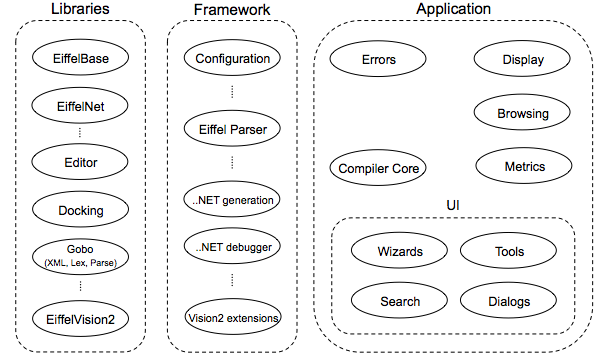
\includegraphics[scale=0.7]{images/eiffelstudio-structure-full.png}
}
\caption[Overview of the EiffelStudio structure]{Overview of the EiffelStudio structure (source: EiffelStudio presentation by Emmanuel Stapf).}
\label{fig:eiffelstudio_structure}
\end{figure}
\subsubsection{Why in a view?}
\label{why_a_view}
EiffelStudio has multiple ways of showing the same code, which is taken care of by the View feature. While viewing a piece of Eiffel source code, you can switch to the interface view, for instance, where you can see the signature, comments and contracts of all the features  of the current class, including inherited ones. This gives the user the ability to overview over the structure of the class, through showing information not normally available, and hiding information that is not relevant to the view. In the case of the interface view, the body of features is hidden to ensure a proper overview and to remove clutter from viewing too many features at once.
\paragraph{}
The function of the textual \textsc{bon} tool is similar to this in many ways. It allows the user to see the code from a textual \textsc{bon} perspective, with the idea of charts (informal) and components (formal) to help giving an overview over the structure of the code. The exact functionality of the \textsc{bon} tool will be discussed in later sections. Due to the similarity between the currently implemented views and the textual \textsc{bon} tool, having this new tool as an added view makes it feel like an integrated part of EiffelStudio, and not some external tool.

\subsection{BON syntax highlighting}